\providecommand{\cbxiiyear}{2021}
\begin{enumerate}[label=\thesubsection.\arabic*, ref=\thesubsection.\theenumi,itemsep=1.5em]

\item The probabilities of solving a specific question independently by $A$ and $B$ are $\frac{1}{3}$ and $\frac{1}{5}$ respectively. If both try to solve the question independently, the probability that the question is solved is
\begin{enumerate}[label=\alph*), itemsep=0pt]
    \begin{multicols}{4}
        \item $\frac{7}{15}$
        \item $\frac{8}{15}$
        \item $\frac{2}{15}$
        \item $\frac{14}{15}$
    \end{multicols}
\end{enumerate}
\hfill (CBSE~XII~\cbxiiyear)
\\
\solution
Let $X_A,X_B\in\cbrak{0,1}$ indicate that $A$ and $B$ solve the question, with PMFs
\begin{align}
\brak{p_A\brak{0},\ p_A\brak{1}} = \brak{\frac{2}{3},\ \frac{1}{3}}, \qquad \brak{p_B\brak{0},\ p_B\brak{1}} = \brak{\frac{4}{5},\ \frac{1}{5}}
\end{align}
From \eqref{eq:EE26BTECH11218-cb12-conv}, the PMF of $S=X_A+X_B$ is the convolution
\begin{align}
\brak{p_S\brak{0},\ p_S\brak{1},\ p_S\brak{2}} = \brak{\frac{8}{15},\ \frac{6}{15},\ \frac{1}{15}}
\end{align}
where $p_S\brak{1} = \frac{2}{3}\cdot\frac{1}{5}+\frac{1}{3}\cdot\frac{4}{5} = \frac{6}{15}$. The question is solved iff $S\ge1$, so
\begin{align}
\pr{S\ge1} = 1-p_S\brak{0} = 1-\frac{8}{15} = \frac{7}{15}
\end{align}
which agrees with \eqref{eq:EE26BTECH11218-cb12-atleast}, $1-\brak{1-\frac{1}{3}}\brak{1-\frac{1}{5}}$. Hence the answer is option (a). The following code verifies this in \figref{fig:EE26BTECH11218-cb12_q1}.
\begin{lstlisting}[frame=single, basicstyle=\rmfamily, escapeinside={(*@}{@*)}]
(*@\makebox[\dimexpr\linewidth-2\fboxsep-2\fboxrule\relax][c]{codes/cbXIIq1.py}@*)
\end{lstlisting}
\begin{figure}[H]
    \centering
    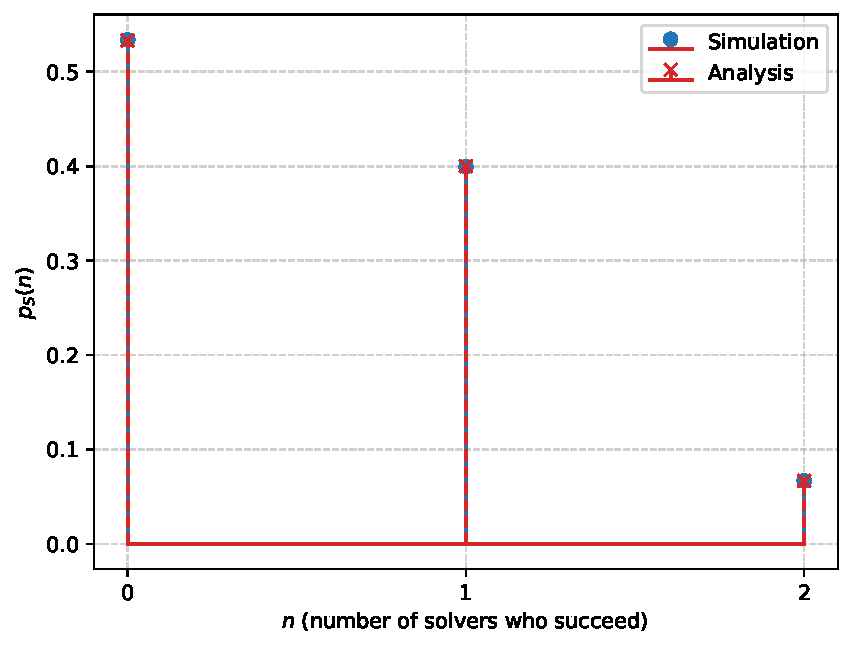
\includegraphics[width=0.70\linewidth]{figs/cbXIIq1.pdf}
    \caption{PMF of the number of solvers who succeed: Simulation vs Analysis}
    \label{fig:EE26BTECH11218-cb12_q1}
\end{figure}
\item If the two lines $L_1: x=5,\ \frac{y}{3-\alpha}=\frac{z}{-2}$ and $L_2: x=2,\ \frac{y}{-1}=\frac{z}{2-\alpha}$ are perpendicular, then the value of $\alpha$ is
\begin{enumerate}[label=\alph*), itemsep=0pt]
    \begin{multicols}{4}
        \item $\frac{2}{3}$
        \item $3$
        \item $4$
        \item $\frac{7}{3}$
    \end{multicols}
\end{enumerate}
\hfill (CBSE~XII~\cbxiiyear)
\\
\solution
From \eqref{eq:EE26BTECH11218-cb12-symm}, the directions of the lines are (the condition $x=5$ or $x=2$ means the $x$ component is $0$)
\begin{align}
\vec{m}_1 = \myvec{0 \\ 3-\alpha \\ -2}, \qquad \vec{m}_2 = \myvec{0 \\ -1 \\ 2-\alpha}
\end{align}
From \eqref{eq:EE26BTECH11218-cb12-perp}, the lines are perpendicular iff
\begin{align}
\vec{m}_1^{\top}\vec{m}_2 = -\brak{3-\alpha}-2\brak{2-\alpha} = 3\alpha-7 = 0 \implies \alpha = \frac{7}{3}
\end{align}
For $\alpha=\frac{2}{3},3,4$ the inner product is $-5,2,5$, all nonzero. Hence the answer is option (d). The following code verifies this in \figref{fig:EE26BTECH11218-cb12_q3}.
\begin{lstlisting}[frame=single, basicstyle=\rmfamily, escapeinside={(*@}{@*)}]
(*@\makebox[\dimexpr\linewidth-2\fboxsep-2\fboxrule\relax][c]{codes/cbXIIq3.py}@*)
\end{lstlisting}
\begin{figure}[H]
    \centering
    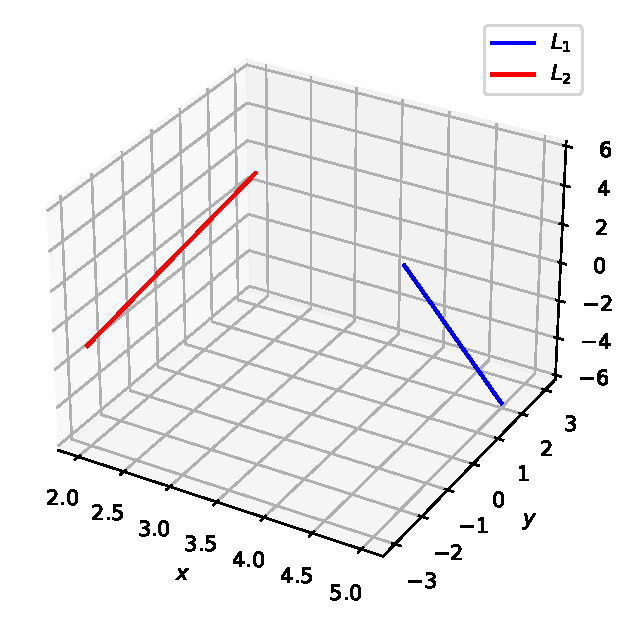
\includegraphics[width=0.70\linewidth]{figs/cbXIIq3.pdf}
    \caption{The perpendicular lines $L_1$ and $L_2$ for $\alpha=\frac{7}{3}$}
    \label{fig:EE26BTECH11218-cb12_q3}
\end{figure}
\item $\displaystyle\int_0^1\tan\brak{\sin^{-1}x}\,dx$ equals
\begin{enumerate}[label=\alph*), itemsep=0pt]
    \begin{multicols}{4}
        \item $2$
        \item $0$
        \item $-1$
        \item $1$
    \end{multicols}
\end{enumerate}
\hfill (CBSE~XII~\cbxiiyear)
\\
\solution
From \eqref{eq:EE26BTECH11218-cb12-improper}, $\tan\brak{\sin^{-1}x}=\frac{x}{\sqrt{1-x^2}}$, which is unbounded as $x\to1^{-}$, so the integral is improper. For $b<1$,
\begin{align}
\int_0^b\frac{x}{\sqrt{1-x^2}}dx = \sbrak{-\sqrt{1-x^2}}_0^b = 1-\sqrt{1-b^2}
\end{align}
and the limit is
\begin{align}
\lim_{b\to1^{-}}\brak{1-\sqrt{1-b^2}} = 1
\end{align}
The substitution $x=\sin\theta$ gives the same value, $\int_0^{\pi/2}\tan\theta\cos\theta\,d\theta=\int_0^{\pi/2}\sin\theta\,d\theta=1$. Hence the answer is option (d). The following code verifies this in \figref{fig:EE26BTECH11218-cb12_q6}.
\begin{lstlisting}[frame=single, basicstyle=\rmfamily, escapeinside={(*@}{@*)}]
(*@\makebox[\dimexpr\linewidth-2\fboxsep-2\fboxrule\relax][c]{codes/cbXIIq6.py}@*)
\end{lstlisting}
\begin{figure}[H]
    \centering
    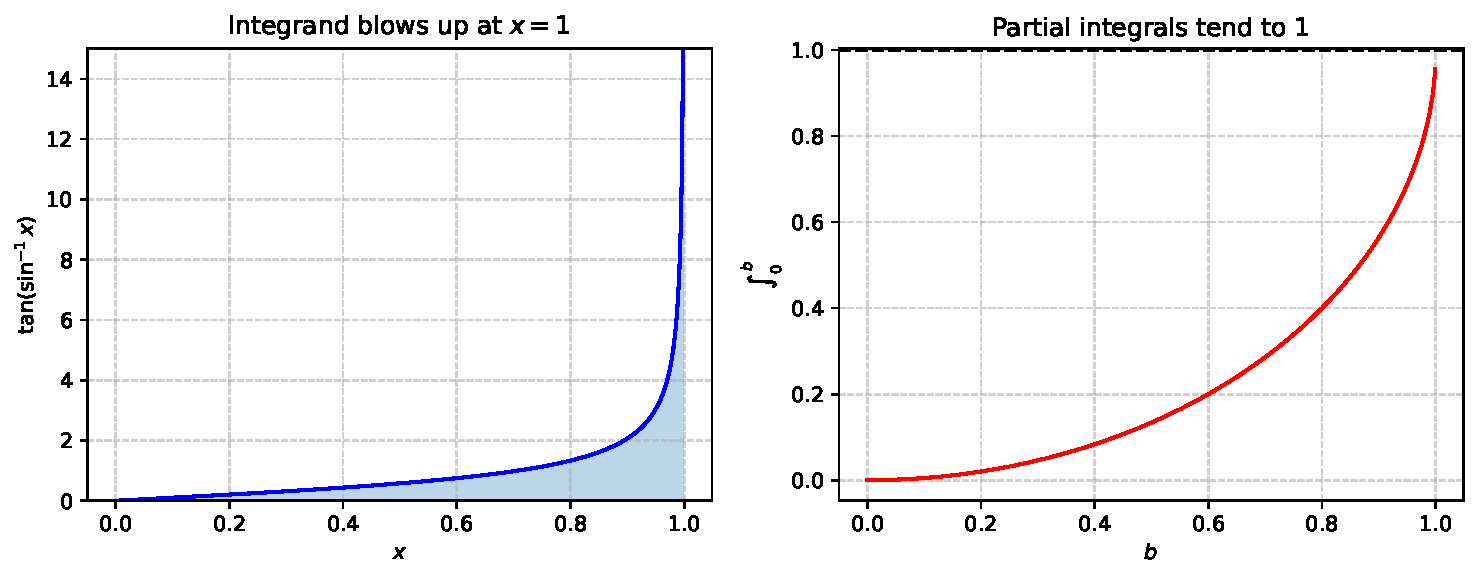
\includegraphics[width=0.95\linewidth]{figs/cbXIIq6.pdf}
    \caption{The integrand and the partial integrals $\int_0^b$ tending to $1$}
    \label{fig:EE26BTECH11218-cb12_q6}
\end{figure}
\item $\displaystyle\int\frac{e^x}{x+1}\sbrak{1+\brak{x+1}\log\brak{x+1}}dx$ equals
\begin{enumerate}[label=\alph*), itemsep=0pt]
    \begin{multicols}{4}
        \item $\frac{e^x}{x+1}+c$
        \item $e^x\frac{x}{x+1}+c$
        \item $e^x\log\brak{x+1}+e^x+c$
        \item $e^x\log\brak{x+1}+c$
    \end{multicols}
\end{enumerate}
\hfill (CBSE~XII~\cbxiiyear)
\\
\solution
The integrand is
\begin{align}
\frac{e^x}{x+1}\sbrak{1+\brak{x+1}\log\brak{x+1}} &= e^x\sbrak{\log\brak{x+1}+\frac{1}{x+1}} \\
&= e^x\brak{f+f'}, \quad f\brak{x}=\log\brak{x+1}
\end{align}
From \eqref{eq:EE26BTECH11218-cb12-expf},
\begin{align}
\int e^x\brak{f+f'}dx = e^xf+c = e^x\log\brak{x+1}+c
\end{align}
Hence the answer is option (d). Numerically, only option (d) has $F\brak{b}-F\brak{0}$ equal to $\int_0^b$ of the integrand (for $b=1$ both are $1.8842$). The following code verifies this in \figref{fig:EE26BTECH11218-cb12_q7}.
\begin{lstlisting}[frame=single, basicstyle=\rmfamily, escapeinside={(*@}{@*)}]
(*@\makebox[\dimexpr\linewidth-2\fboxsep-2\fboxrule\relax][c]{codes/cbXIIq7.py}@*)
\end{lstlisting}
\begin{figure}[H]
    \centering
    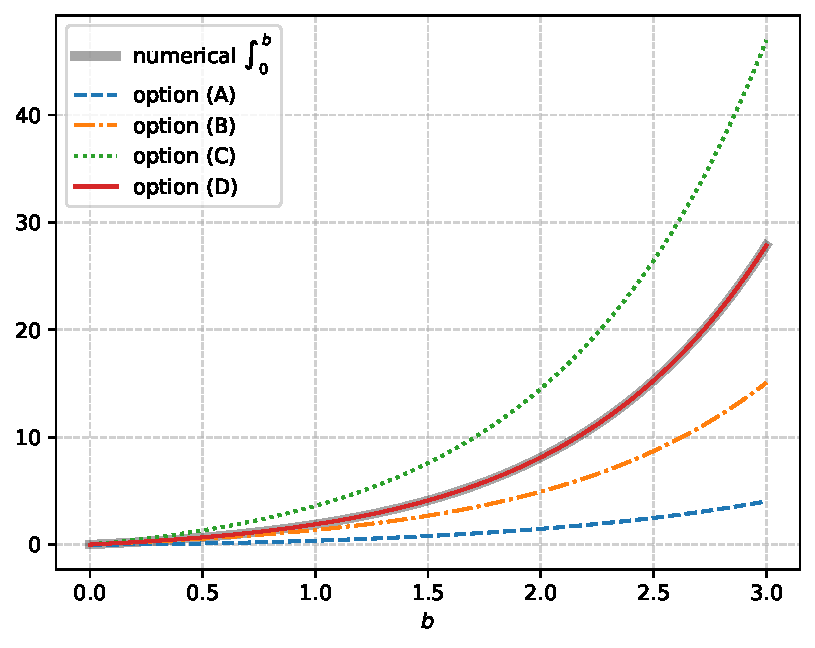
\includegraphics[width=0.70\linewidth]{figs/cbXIIq7.pdf}
    \caption{Numerical $\int_0^b$ compared with the increments of the four options}
    \label{fig:EE26BTECH11218-cb12_q7}
\end{figure}
\item The integrating factor of the differential equation $x\diff{y}{x}-y=\log x$ is \underline{\hspace{2cm}}.
\hfill (CBSE~XII~\cbxiiyear)
\\
\solution
In the form $\diff{y}{x}+Py=Q$ we have $P=-\frac{1}{x}$ and $Q=\frac{\log x}{x}$. From \eqref{eq:EE26BTECH11218-cb12-linode},
\begin{align}
\mu\brak{x} = e^{\int P\,dx} = e^{-\log x} = \frac{1}{x}
\end{align}
Then $\diff{}{x}\brak{\frac{y}{x}}=\frac{\log x}{x^2}$, and integrating by parts,
\begin{align}
\frac{y}{x} = -\frac{\log x+1}{x}+C \implies y = -\log x-1+Cx
\end{align}
The integrating factor is $\frac{1}{x}$. The following code verifies this with a numerical solution of the ODE in \figref{fig:EE26BTECH11218-cb12_q14}.
\begin{lstlisting}[frame=single, basicstyle=\rmfamily, escapeinside={(*@}{@*)}]
(*@\makebox[\dimexpr\linewidth-2\fboxsep-2\fboxrule\relax][c]{codes/cbXIIq14.py}@*)
\end{lstlisting}
\begin{figure}[H]
    \centering
    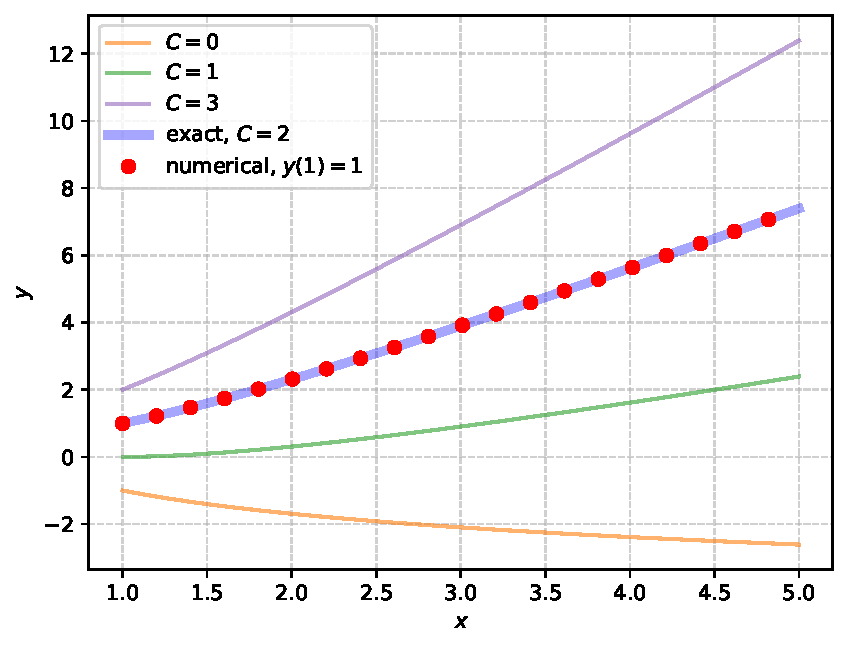
\includegraphics[width=0.70\linewidth]{figs/cbXIIq14.pdf}
    \caption{Numerical solution with $y\brak{1}=1$ (so $C=2$) against the closed form}
    \label{fig:EE26BTECH11218-cb12_q14}
\end{figure}
\item From a pack of $52$ cards, $3$ cards are drawn at random (without replacement). The probability that they are two red cards and one black card is \underline{\hspace{2cm}}.
\hfill (CBSE~XII~\cbxiiyear)
\\
\solution
Let $X$ be the number of red cards among the three drawn. From \eqref{eq:EE26BTECH11218-cb12-hyper} with $M=52$, $K=26$, $n=3$,
\begin{align}
\pr{X=2} = \frac{\binom{26}{2}\binom{26}{1}}{\binom{52}{3}} = \frac{325\times26}{22100} = \frac{13}{34}
\end{align}
The complete PMF is
\begin{align}
\brak{p_X\brak{0},\ p_X\brak{1},\ p_X\brak{2},\ p_X\brak{3}} = \brak{\frac{2}{17},\ \frac{13}{34},\ \frac{13}{34},\ \frac{2}{17}}
\end{align}
which sums to $1$. The following code verifies this in \figref{fig:EE26BTECH11218-cb12_q15}.
\begin{lstlisting}[frame=single, basicstyle=\rmfamily, escapeinside={(*@}{@*)}]
(*@\makebox[\dimexpr\linewidth-2\fboxsep-2\fboxrule\relax][c]{codes/cbXIIq15.py}@*)
\end{lstlisting}
\begin{figure}[H]
    \centering
    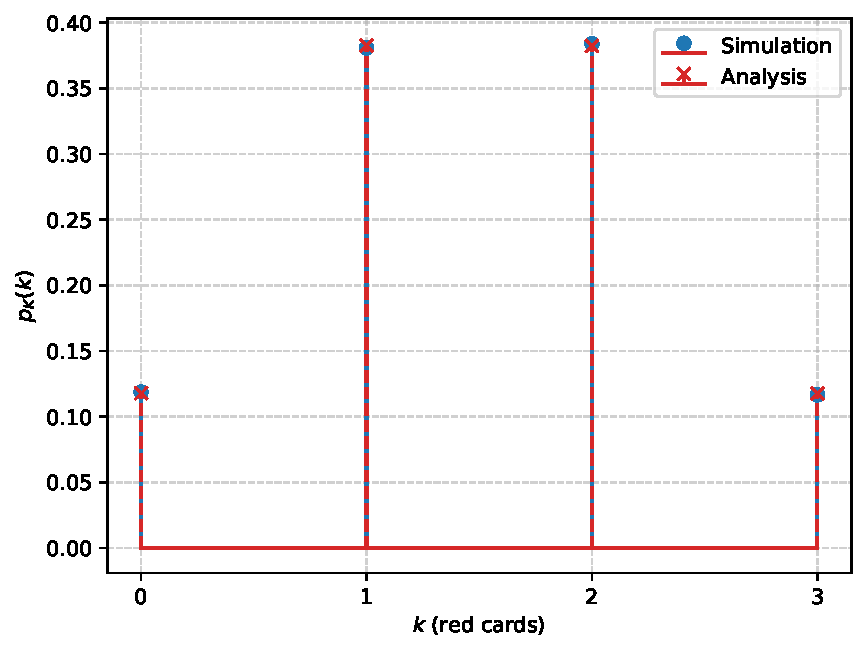
\includegraphics[width=0.70\linewidth]{figs/cbXIIq15.pdf}
    \caption{PMF of the number of red cards in three draws: Simulation vs Analysis}
    \label{fig:EE26BTECH11218-cb12_q15}
\end{figure}
\item If $\myvec{4 & x+2 \\ 2x-3 & x+1}$ is a symmetric matrix, then find the value of $x$.
\hfill (CBSE~XII~\cbxiiyear)
\\
\solution
Let the matrix be $\vec{A}$. From \eqref{eq:EE26BTECH11218-cb12-symskew}, the skew-symmetric part is
\begin{align}
\vec{K} = \frac{\vec{A}-\vec{A}^{\top}}{2} = \frac{5-x}{2}\myvec{0 & 1 \\ -1 & 0}
\end{align}
since $\brak{x+2}-\brak{2x-3}=5-x$. The matrix is symmetric iff $\vec{K}=\vec{0}$,
\begin{align}
5-x=0 \implies x=5, \qquad \vec{A} = \myvec{4 & 7 \\ 7 & 6}
\end{align}
The following code verifies this in \figref{fig:EE26BTECH11218-cb12_q19a}.
\begin{lstlisting}[frame=single, basicstyle=\rmfamily, escapeinside={(*@}{@*)}]
(*@\makebox[\dimexpr\linewidth-2\fboxsep-2\fboxrule\relax][c]{codes/cbXIIq19a.py}@*)
\end{lstlisting}
\begin{figure}[H]
    \centering
    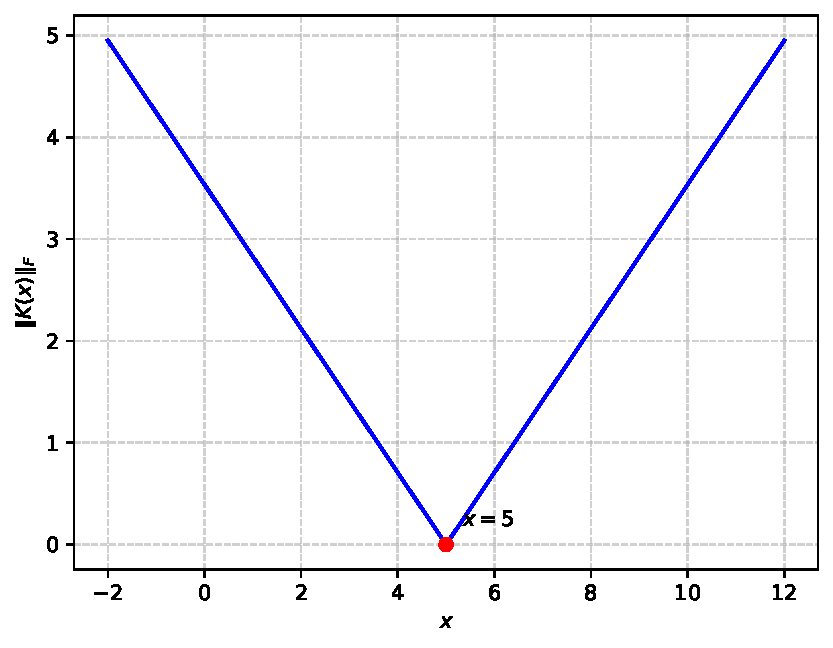
\includegraphics[width=0.70\linewidth]{figs/cbXIIq19a.pdf}
    \caption{Norm of the skew-symmetric part $\vec{K}\brak{x}$, zero at $x=5$}
    \label{fig:EE26BTECH11218-cb12_q19a}
\end{figure}
\item If $\vec{A}$ is a square matrix such that $\vec{A}^2=\vec{A}$, then find $\brak{2\vec{I}+\vec{A}}^3-19\vec{A}$.
\hfill (CBSE~XII~\cbxiiyear)
\\
\solution
Let $p\brak{\lambda}=\brak{2+\lambda}^3-19\lambda=\lambda^3+6\lambda^2-7\lambda+8$. Dividing by $\lambda^2-\lambda$,
\begin{align}
p\brak{\lambda} = \brak{\lambda^2-\lambda}\brak{\lambda+7}+8
\end{align}
so $r_1=0$ and $r_0=8$. Since $\vec{A}^2-\vec{A}=\vec{0}$, from \eqref{eq:EE26BTECH11218-cb12-idem},
\begin{align}
\brak{2\vec{I}+\vec{A}}^3-19\vec{A} = \brak{\vec{A}^2-\vec{A}}\brak{\vec{A}+7\vec{I}}+8\vec{I} = 8\vec{I}
\end{align}
This agrees with the eigenvalues of $\vec{A}$ being $0$ or $1$, where $p\brak{0}=p\brak{1}=8$. The following code verifies this for an orthogonal and an oblique projection matrix in \figref{fig:EE26BTECH11218-cb12_q19b}.
\begin{lstlisting}[frame=single, basicstyle=\rmfamily, escapeinside={(*@}{@*)}]
(*@\makebox[\dimexpr\linewidth-2\fboxsep-2\fboxrule\relax][c]{codes/cbXIIq19b.py}@*)
\end{lstlisting}
\begin{figure}[H]
    \centering
    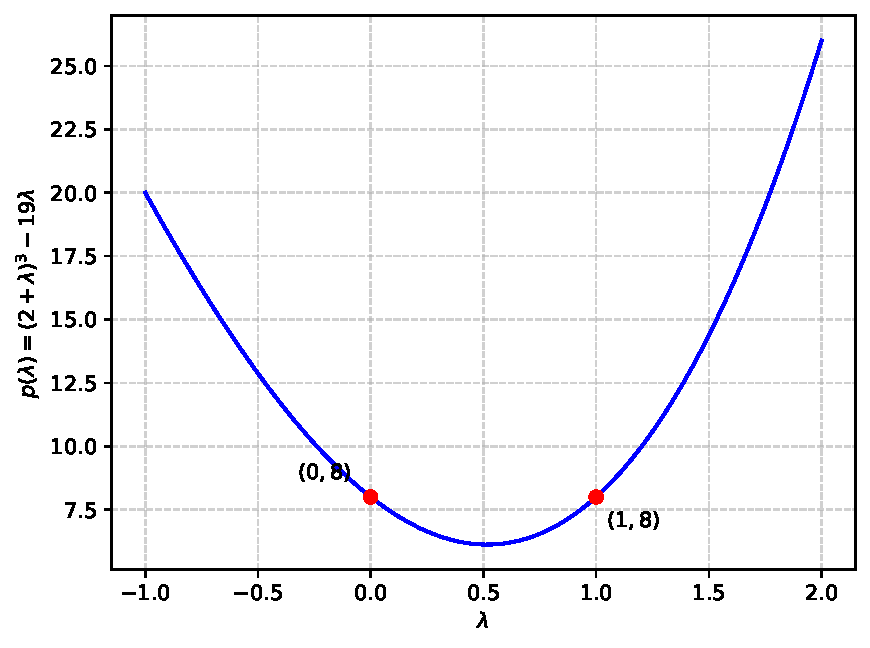
\includegraphics[width=0.70\linewidth]{figs/cbXIIq19b.pdf}
    \caption{$p\brak{\lambda}=\brak{2+\lambda}^3-19\lambda$ takes the value $8$ at $\lambda=0$ and $\lambda=1$}
    \label{fig:EE26BTECH11218-cb12_q19b}
\end{figure}
\item Let $W$ denote the set of words in the English dictionary. Define the relation $R$ by $R=\cbrak{\brak{x,y}\in W\times W : x \text{ and } y \text{ have at least one letter in common}}$. Show that $R$ is reflexive and symmetric, but not transitive.
\hfill (CBSE~XII~\cbxiiyear)
\\
\solution
From \eqref{eq:EE26BTECH11218-cb12-relation}, take $\vec{M}=\brak{\vec{L}\vec{L}^{\top}>0}$, where $L_{ik}=1$ iff word $i$ contains letter $k$.
\begin{enumerate}
\item \textbf{Reflexive:} $\brak{\vec{L}\vec{L}^{\top}}_{ii}=\sum_kL_{ik}^2$ is the number of distinct letters of word $i$, which is at least $1$ for every word, so $M_{ii}=1$.
\item \textbf{Symmetric:} $\vec{L}\vec{L}^{\top}$ is symmetric, so $\vec{M}=\vec{M}^{\top}$.
\item \textbf{Not transitive:} take $x=$ ``at'', $y=$ ``tip'', $z=$ ``pin''. The words ``at'' and ``tip'' share $t$, and ``tip'' and ``pin'' share $i,p$, so $\brak{\vec{M}^2}_{xz}>0$. But ``at'' and ``pin'' have no common letter, so $M_{xz}=0$ and $\brak{\vec{M}^2>0}\not\subseteq\brak{\vec{M}>0}$.
\end{enumerate}
The following code verifies this on a small set of words in \figref{fig:EE26BTECH11218-cb12_q21a}.
\begin{lstlisting}[frame=single, basicstyle=\rmfamily, escapeinside={(*@}{@*)}]
(*@\makebox[\dimexpr\linewidth-2\fboxsep-2\fboxrule\relax][c]{codes/cbXIIq21a.py}@*)
\end{lstlisting}
\begin{figure}[H]
    \centering
    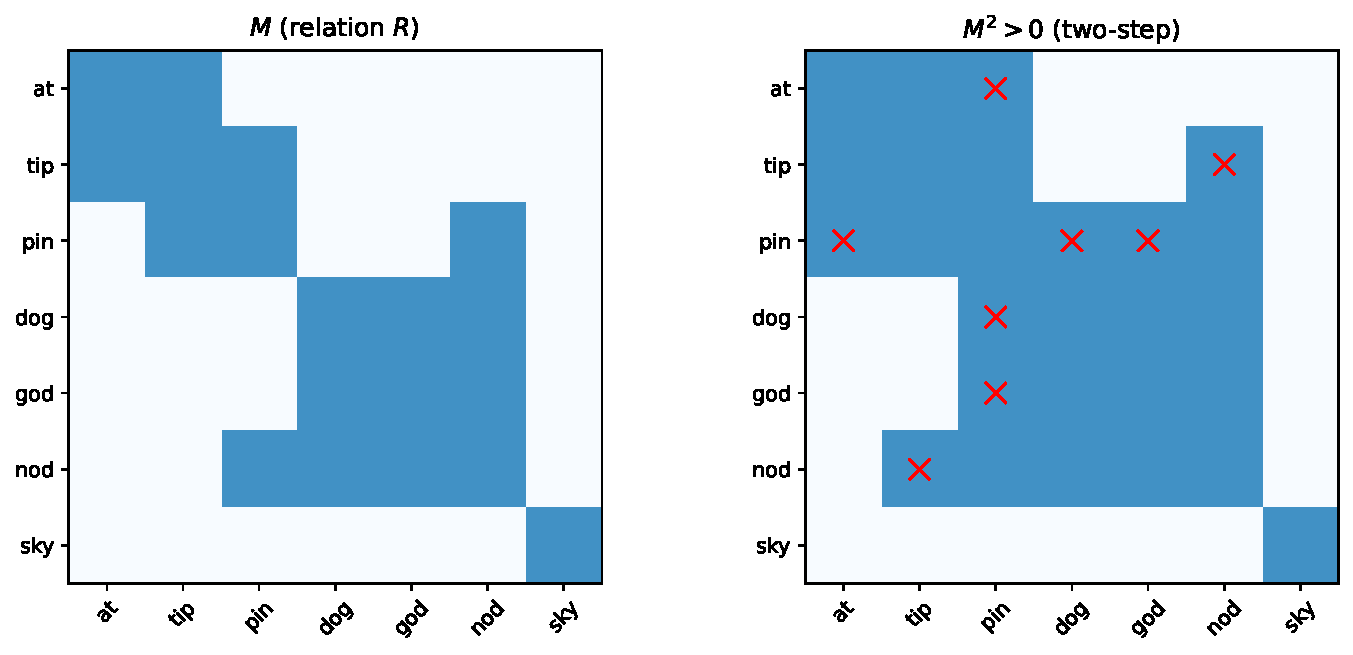
\includegraphics[width=0.85\linewidth]{figs/cbXIIq21a.pdf}
    \caption{$\vec{M}$ and $\brak{\vec{M}^2>0}$ for a few words; crosses mark violations of transitivity}
    \label{fig:EE26BTECH11218-cb12_q21a}
\end{figure}
\item For the matrix $\vec{A}=\myvec{2 & 3 \\ -4 & -6}$, verify $\vec{A}\brak{\mathrm{adj}\,\vec{A}} = \brak{\mathrm{adj}\,\vec{A}}\vec{A} = \abs{\vec{A}}\vec{I}$.
\hfill (CBSE~XII~\cbxiiyear)
\\
\solution
Here $\mathrm{tr}\brak{\vec{A}} = 2-6 = -4$ and $\abs{\vec{A}} = -12+12 = 0$, so $\vec{A}$ is singular and the inverse formula cannot be used. From \eqref{eq:EE26BTECH11218-cb12-ch}, Cayley-Hamilton gives
\begin{align}
\vec{A}^2+4\vec{A} = \vec{0}
\end{align}
(which can be checked directly: $\vec{A}^2=\myvec{-8 & -12 \\ 16 & 24}=-4\vec{A}$). From \eqref{eq:EE26BTECH11218-cb12-adj},
\begin{align}
\mathrm{adj}\,\vec{A} = -4\vec{I}-\vec{A} = \myvec{-6 & -3 \\ 4 & 2}
\end{align}
which is the transposed cofactor matrix. Then
\begin{align}
\vec{A}\brak{\mathrm{adj}\,\vec{A}} &= -4\vec{A}-\vec{A}^2 = -\brak{\vec{A}^2+4\vec{A}} = \vec{0} = \abs{\vec{A}}\vec{I} \\
\brak{\mathrm{adj}\,\vec{A}}\vec{A} &= -4\vec{A}-\vec{A}^2 = \vec{0} = \abs{\vec{A}}\vec{I}
\end{align}
Geometrically, the columns of $\mathrm{adj}\,\vec{A}$ are multiples of $\brak{3,\ -2}^{\top}$, which spans the null space of $\vec{A}$, so $\vec{A}$ maps them to $\vec{0}$. The following code verifies this in \figref{fig:EE26BTECH11218-cb12_q22}.
\begin{lstlisting}[frame=single, basicstyle=\rmfamily, escapeinside={(*@}{@*)}]
(*@\makebox[\dimexpr\linewidth-2\fboxsep-2\fboxrule\relax][c]{codes/cbXIIq22.py}@*)
\end{lstlisting}
\begin{figure}[H]
    \centering
    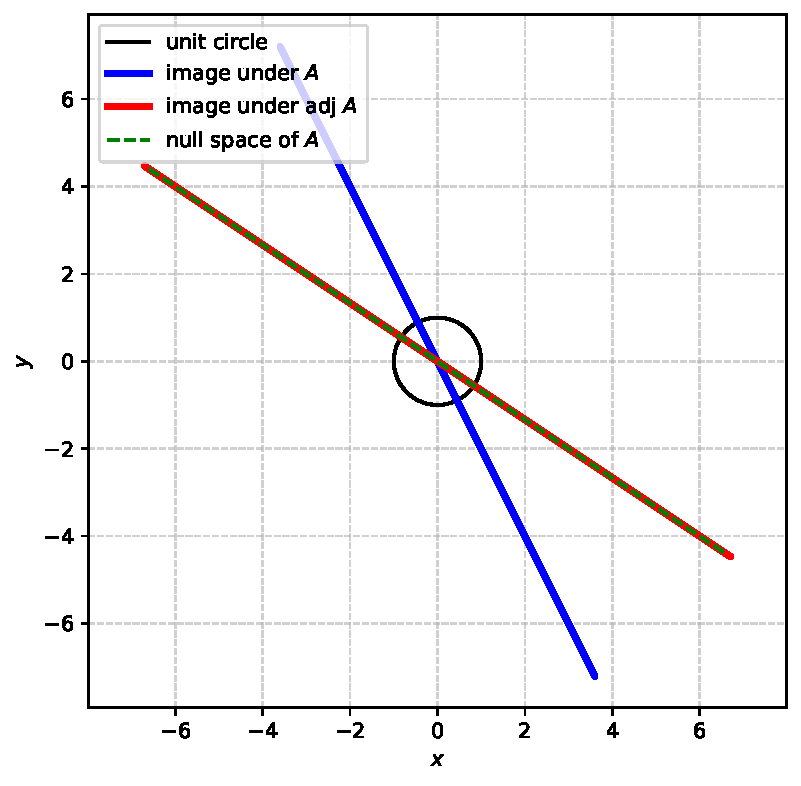
\includegraphics[width=0.70\linewidth]{figs/cbXIIq22.pdf}
    \caption{Images of the unit circle under $\vec{A}$ and $\mathrm{adj}\,\vec{A}$; the latter lies in the null space of $\vec{A}$}
    \label{fig:EE26BTECH11218-cb12_q22}
\end{figure}
\item A bag contains $19$ tickets numbered $1$ to $19$. A ticket is drawn at random and then another ticket is drawn without replacing the first one. Find the probability distribution of the number of even numbers on the tickets.
\hfill (CBSE~XII~\cbxiiyear)
\\
\solution
Let $X$ be the number of even tickets. Among $1,\dots,19$ there are $9$ even and $10$ odd tickets, so from \eqref{eq:EE26BTECH11218-cb12-hyper} with $M=19$, $K=9$, $n=2$,
\begin{align}
p_X\brak{k} = \frac{\binom{9}{k}\binom{10}{2-k}}{\binom{19}{2}}, \quad \binom{19}{2}=171
\end{align}
\begin{center}
\begin{tabular}{|c|c|c|c|}
\hline
$k$ & $0$ & $1$ & $2$ \\ \hline
$p_X\brak{k}$ & $\frac{45}{171}=\frac{5}{19}$ & $\frac{90}{171}=\frac{10}{19}$ & $\frac{36}{171}=\frac{4}{19}$ \\ \hline
\end{tabular}
\end{center}
The probabilities sum to $1$, and the mean is $E\sbrak{X}=\frac{2\cdot9}{19}=\frac{18}{19}$. The following code verifies this in \figref{fig:EE26BTECH11218-cb12_q26a}.
\begin{lstlisting}[frame=single, basicstyle=\rmfamily, escapeinside={(*@}{@*)}]
(*@\makebox[\dimexpr\linewidth-2\fboxsep-2\fboxrule\relax][c]{codes/cbXIIq26a.py}@*)
\end{lstlisting}
\begin{figure}[H]
    \centering
    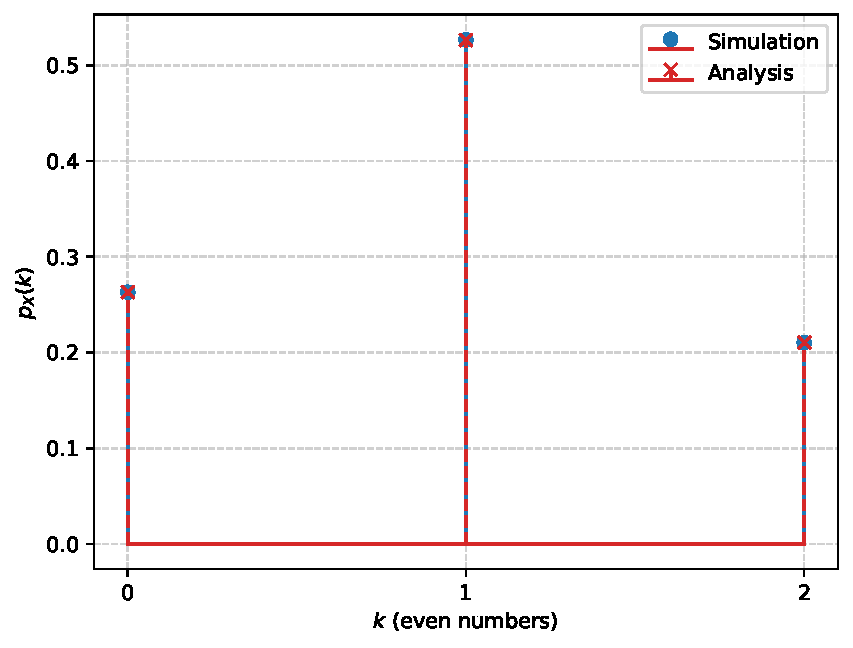
\includegraphics[width=0.70\linewidth]{figs/cbXIIq26a.pdf}
    \caption{PMF of the number of even tickets: Simulation vs Analysis}
    \label{fig:EE26BTECH11218-cb12_q26a}
\end{figure}
\item Find the probability distribution of the number of successes in two tosses of a die, where a success is defined as ``number greater than $5$''.
\hfill (CBSE~XII~\cbxiiyear)
\\
\solution
A success is the face $6$, so $p=\frac{1}{6}$. Let $X$ be the number of successes in $n=2$ independent tosses. From \eqref{eq:EE26BTECH11218-cb12-binom},
\begin{align}
p_X\brak{k} = \binom{2}{k}\brak{\frac{1}{6}}^k\brak{\frac{5}{6}}^{2-k}
\end{align}
\begin{center}
\begin{tabular}{|c|c|c|c|}
\hline
$k$ & $0$ & $1$ & $2$ \\ \hline
$p_X\brak{k}$ & $\frac{25}{36}$ & $\frac{10}{36}=\frac{5}{18}$ & $\frac{1}{36}$ \\ \hline
\end{tabular}
\end{center}
This is also the convolution $\brak{\frac{5}{6},\ \frac{1}{6}}*\brak{\frac{5}{6},\ \frac{1}{6}}$, with mean $np=\frac{1}{3}$ and variance $np\brak{1-p}=\frac{5}{18}$. The following code verifies this in \figref{fig:EE26BTECH11218-cb12_q26b}.
\begin{lstlisting}[frame=single, basicstyle=\rmfamily, escapeinside={(*@}{@*)}]
(*@\makebox[\dimexpr\linewidth-2\fboxsep-2\fboxrule\relax][c]{codes/cbXIIq26b.py}@*)
\end{lstlisting}
\begin{figure}[H]
    \centering
    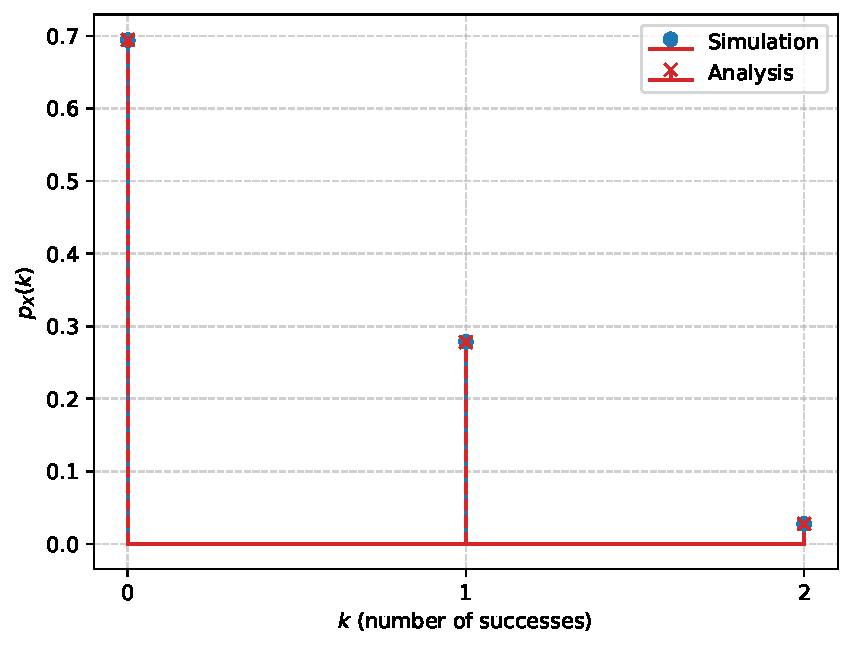
\includegraphics[width=0.70\linewidth]{figs/cbXIIq26b.pdf}
    \caption{PMF of the number of sixes in two tosses: Simulation vs Analysis}
    \label{fig:EE26BTECH11218-cb12_q26b}
\end{figure}
\item Find the equation of the line joining $A\brak{1,3}$ and $B\brak{0,0}$ using determinants. Also find $k$ if $D\brak{k,0}$ is a point such that the area of $\triangle ABD$ is $3$ square units.
\hfill (CBSE~XII~\cbxiiyear)
\\
\solution
From \eqref{eq:EE26BTECH11218-cb12-det}, the line $AB$ is
\begin{align}
\mydet{x & y & 1 \\ 1 & 3 & 1 \\ 0 & 0 & 1} = x\brak{3-0}-y\brak{1-0}+1\brak{0-0} = 3x-y = 0
\end{align}
The area of $\triangle ABD$ is
\begin{align}
\Delta = \frac{1}{2}\abs{\mydet{1 & 3 & 1 \\ 0 & 0 & 1 \\ k & 0 & 1}} = \frac{1}{2}\abs{3k} = 3 \implies \abs{k}=2
\end{align}
\begin{align}
\therefore k = \pm2
\end{align}
The following code verifies this in \figref{fig:EE26BTECH11218-cb12_q28b}.
\begin{lstlisting}[frame=single, basicstyle=\rmfamily, escapeinside={(*@}{@*)}]
(*@\makebox[\dimexpr\linewidth-2\fboxsep-2\fboxrule\relax][c]{codes/cbXIIq28b.py}@*)
\end{lstlisting}
\begin{figure}[H]
    \centering
    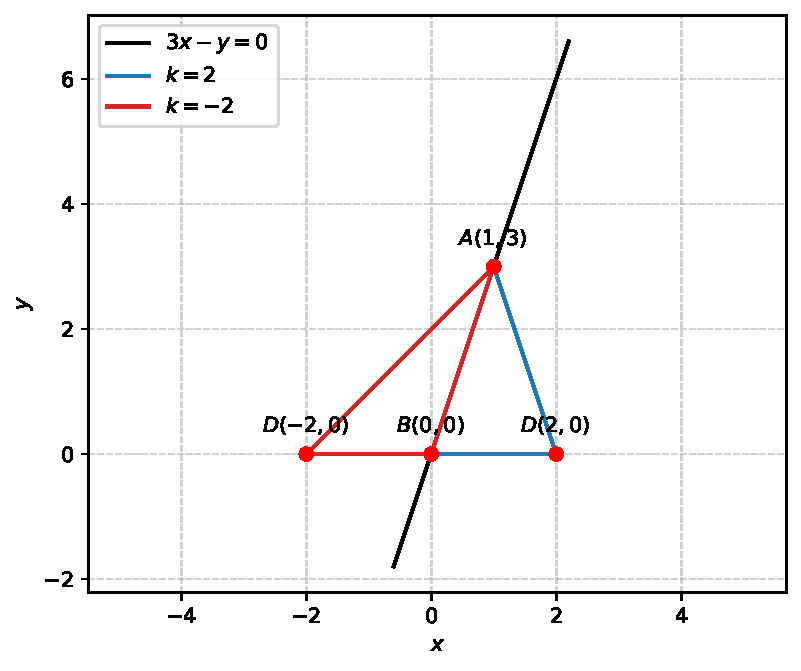
\includegraphics[width=0.70\linewidth]{figs/cbXIIq28b.pdf}
    \caption{The line $3x-y=0$ and the triangles $ABD$ for $k=\pm2$}
    \label{fig:EE26BTECH11218-cb12_q28b}
\end{figure}
\item Prove that three points $A$, $B$ and $C$ with position vectors $\vec{a}$, $\vec{b}$ and $\vec{c}$ respectively are collinear if and only if $\brak{\vec{b}\times\vec{c}}+\brak{\vec{c}\times\vec{a}}+\brak{\vec{a}\times\vec{b}}=\vec{0}$.
\hfill (CBSE~XII~\cbxiiyear)
\\
\solution
Let $\vec{S}=\vec{b}\times\vec{c}+\vec{c}\times\vec{a}+\vec{a}\times\vec{b}$. From \eqref{eq:EE26BTECH11218-cb12-cross},
\begin{align}
\vec{S} = \brak{\vec{b}-\vec{a}}\times\brak{\vec{c}-\vec{a}}
\end{align}
This vanishes iff $\vec{b}-\vec{a}$ and $\vec{c}-\vec{a}$ are parallel, that is (for $A\ne B$) iff $\vec{c}-\vec{a}=\kappa\brak{\vec{b}-\vec{a}}$ for some $\kappa$, which says that $C$ lies on the line $AB$. If $A=B$ both statements hold trivially. Hence $A,B,C$ are collinear iff $\vec{S}=\vec{0}$. Moreover $\norm{\vec{S}}=2\,\mathrm{area}\brak{\triangle ABC}$.

For $\vec{a}=\brak{1,\ 0,\ 2}^{\top}$ and $\vec{b}=\brak{3,\ 1,\ 1}^{\top}$, the point $\vec{c}=\vec{a}+2.5\brak{\vec{b}-\vec{a}}$ gives $\vec{S}=\vec{0}$, while $\vec{c}=\brak{2,\ 3,\ 4}^{\top}$ gives $\vec{S}=\brak{5,\ -5,\ 5}^{\top}$ and $\frac{1}{2}\norm{\vec{S}}=4.33$, which equals the area from Heron's formula. The following code verifies this in \figref{fig:EE26BTECH11218-cb12_q29}.
\begin{lstlisting}[frame=single, basicstyle=\rmfamily, escapeinside={(*@}{@*)}]
(*@\makebox[\dimexpr\linewidth-2\fboxsep-2\fboxrule\relax][c]{codes/cbXIIq29.py}@*)
\end{lstlisting}
\begin{figure}[H]
    \centering
    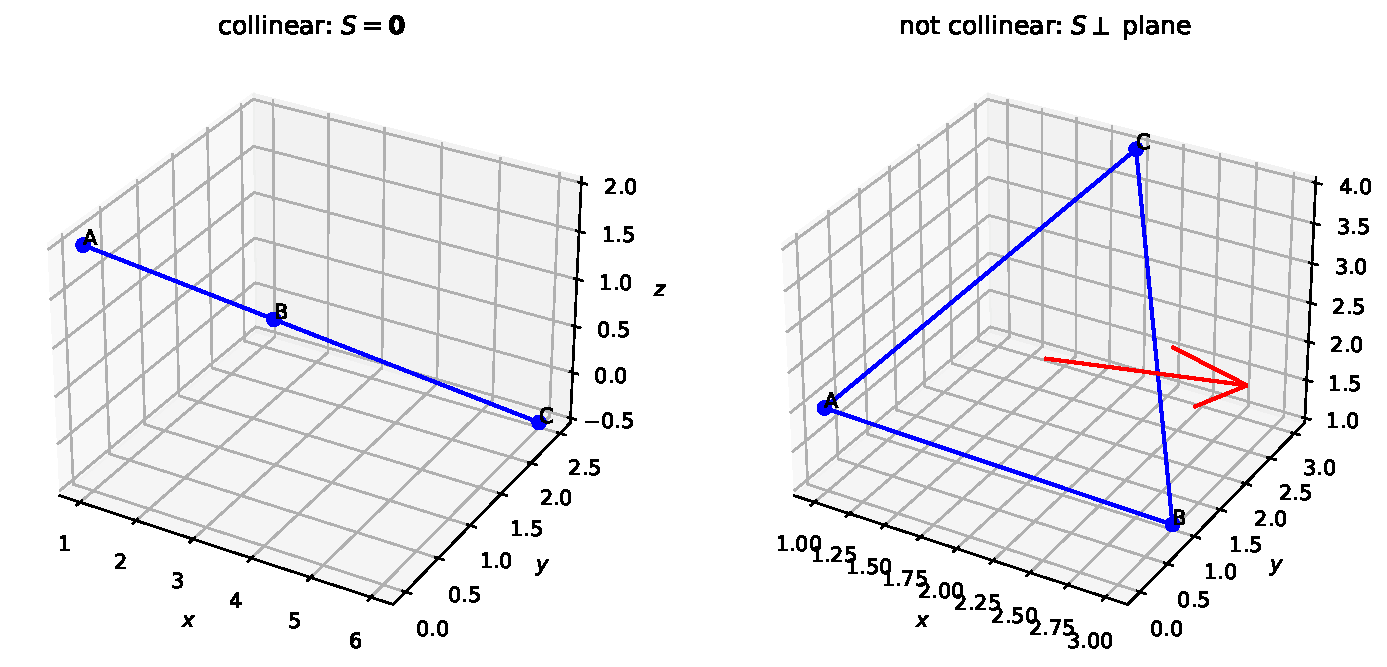
\includegraphics[width=0.95\linewidth]{figs/cbXIIq29.pdf}
    \caption{Collinear points ($\vec{S}=\vec{0}$) and a triangle with $\vec{S}$ normal to its plane}
    \label{fig:EE26BTECH11218-cb12_q29}
\end{figure}
\item Find the shortest distance between the lines $\frac{x-1}{2}=\frac{y+1}{3}=z$ and $\frac{x+1}{5}=\frac{y-2}{1},\ z=2$, and hence write whether the lines are intersecting or not.
\hfill (CBSE~XII~\cbxiiyear)
\\
\solution
From \eqref{eq:EE26BTECH11218-cb12-symm}, the lines are $\vec{x}=\vec{a}_1+s\vec{m}_1$ and $\vec{x}=\vec{a}_2+t\vec{m}_2$ with
\begin{align}
\vec{a}_1 = \myvec{1 \\ -1 \\ 0}, \ \vec{m}_1 = \myvec{2 \\ 3 \\ 1}, \qquad &\vec{a}_2 = \myvec{-1 \\ 2 \\ 2}, \ \vec{m}_2 = \myvec{5 \\ 1 \\ 0} \\
\vec{b} = \vec{a}_2-\vec{a}_1 &= \myvec{-2 \\ 3 \\ 2}
\end{align}
The normal equations in \eqref{eq:EE26BTECH11218-cb12-skew} are
\begin{align}
\myvec{14 & 13 \\ 13 & 26}\myvec{s \\ -t} = \myvec{7 \\ -7} \implies s=\frac{7}{5}, \quad t=\frac{63}{65}
\end{align}
The closest points are $\brak{3.8,\ 3.2,\ 1.4}^{\top}$ on the first line and $\brak{3.846,\ 2.969,\ 2}^{\top}$ on the second. The distance is $\norm{\vec{M}\vec{z}-\vec{b}}$, and from \eqref{eq:EE26BTECH11218-cb12-skew-cross}, with $\vec{m}_1\times\vec{m}_2=\brak{-1,\ 5,\ -13}^{\top}$ and $\vec{b}^{\top}\brak{\vec{m}_1\times\vec{m}_2}=-9$,
\begin{align}
d = \frac{\abs{-9}}{\sqrt{195}} = \frac{9}{\sqrt{195}} \approx 0.645
\end{align}
Since $d\ne0$, the lines do \textbf{not} intersect (they are skew). The following code verifies this in \figref{fig:EE26BTECH11218-cb12_q30a}.
\begin{lstlisting}[frame=single, basicstyle=\rmfamily, escapeinside={(*@}{@*)}]
(*@\makebox[\dimexpr\linewidth-2\fboxsep-2\fboxrule\relax][c]{codes/cbXIIq30a.py}@*)
\end{lstlisting}
\begin{figure}[H]
    \centering
    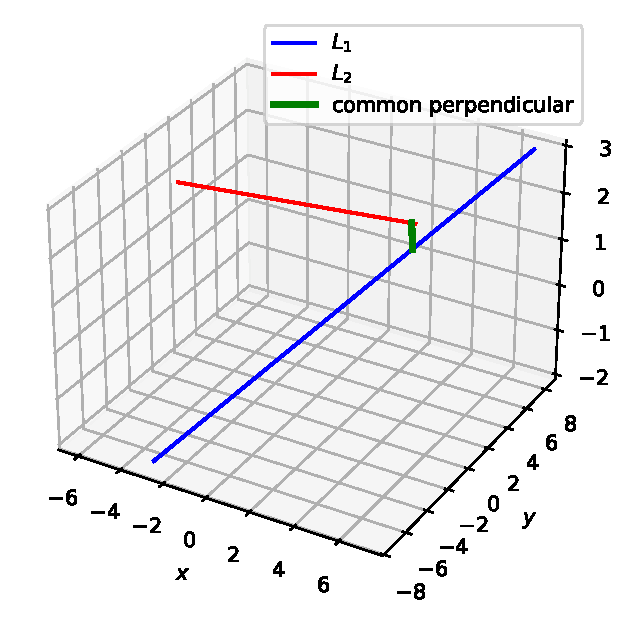
\includegraphics[width=0.80\linewidth]{figs/cbXIIq30a.pdf}
    \caption{Skew lines and their common perpendicular}
    \label{fig:EE26BTECH11218-cb12_q30a}
\end{figure}
\item Find the equation of the plane through the line of intersection of the planes $\vec{r}\cdot\brak{\hat{i}+3\hat{j}}+6=0$ and $\vec{r}\cdot\brak{3\hat{i}-\hat{j}-4\hat{k}}=0$, which is at a unit distance from the origin.
\hfill (CBSE~XII~\cbxiiyear)
\\
\solution
The planes are $\vec{n}_1^{\top}\vec{x}+e_1=0$ and $\vec{n}_2^{\top}\vec{x}+e_2=0$ with
\begin{align}
\vec{n}_1 = \myvec{1 \\ 3 \\ 0}, \ e_1=6, \qquad \vec{n}_2 = \myvec{3 \\ -1 \\ -4}, \ e_2=0
\end{align}
From \eqref{eq:EE26BTECH11218-cb12-pencil}, the planes through the line of intersection have $\vec{n}=\vec{n}_1+\lambda\vec{n}_2$ and $e=6$. From \eqref{eq:EE26BTECH11218-cb12-plane-dist}, the distance from the origin is $1$ iff $\norm{\vec{n}}^2=e^2$,
\begin{align}
\norm{\vec{n}_1+\lambda\vec{n}_2}^2 = \vec{n}_1^{\top}\vec{n}_1+2\lambda\vec{n}_1^{\top}\vec{n}_2+\lambda^2\vec{n}_2^{\top}\vec{n}_2 = 10+0+26\lambda^2 = 36 \implies \lambda=\pm1
\end{align}
\begin{align}
\lambda=1: \ 4x+2y-4z+6=0 \implies 2x+y-2z+3=0 \\
\lambda=-1: \ -2x+4y+4z+6=0 \implies x-2y-2z-3=0
\end{align}
Both are at distance $\frac{3}{3}=1$ from the origin. The following code verifies this in \figref{fig:EE26BTECH11218-cb12_q30b}.
\begin{lstlisting}[frame=single, basicstyle=\rmfamily, escapeinside={(*@}{@*)}]
(*@\makebox[\dimexpr\linewidth-2\fboxsep-2\fboxrule\relax][c]{codes/cbXIIq30b.py}@*)
\end{lstlisting}
\begin{figure}[H]
    \centering
    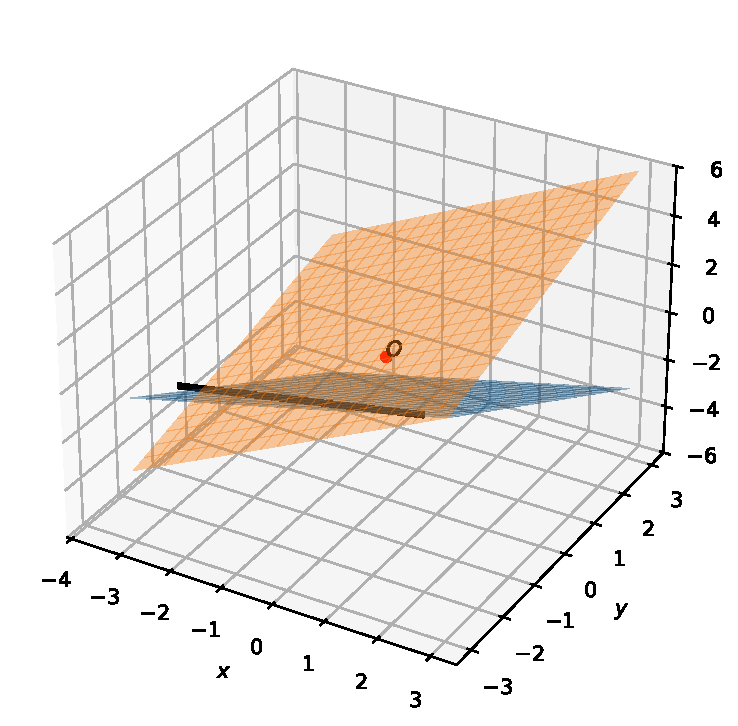
\includegraphics[width=0.80\linewidth]{figs/cbXIIq30b.pdf}
    \caption{The two required planes and the line of intersection of the given planes}
    \label{fig:EE26BTECH11218-cb12_q30b}
\end{figure}
\item A bag contains $5$ red and $4$ black balls, and a second bag contains $3$ red and $6$ black balls. One of the two bags is selected at random and two balls are drawn at random (without replacement), both of which are found to be red. Find the probability that these two balls are drawn from the second bag.
\hfill (CBSE~XII~\cbxiiyear)
\\
\solution
Let $B_i$ be the event that bag $i$ is chosen, with $\pr{B_i}=\frac{1}{2}$, and let $E$ be the event that both balls are red. From \eqref{eq:EE26BTECH11218-cb12-hyper},
\begin{align}
\pr{E\mid B_1} = \frac{\binom{5}{2}}{\binom{9}{2}} = \frac{10}{36}, \qquad \pr{E\mid B_2} = \frac{\binom{3}{2}}{\binom{9}{2}} = \frac{3}{36}
\end{align}
From \eqref{eq:EE26BTECH11218-cb12-bayes},
\begin{align}
\pr{B_2\mid E} = \frac{\frac{1}{2}\cdot\frac{3}{36}}{\frac{1}{2}\cdot\frac{10}{36}+\frac{1}{2}\cdot\frac{3}{36}} = \frac{3}{13}
\end{align}
The following code verifies this in \figref{fig:EE26BTECH11218-cb12_q32}.
\begin{lstlisting}[frame=single, basicstyle=\rmfamily, escapeinside={(*@}{@*)}]
(*@\makebox[\dimexpr\linewidth-2\fboxsep-2\fboxrule\relax][c]{codes/cbXIIq32.py}@*)
\end{lstlisting}
\begin{figure}[H]
    \centering
    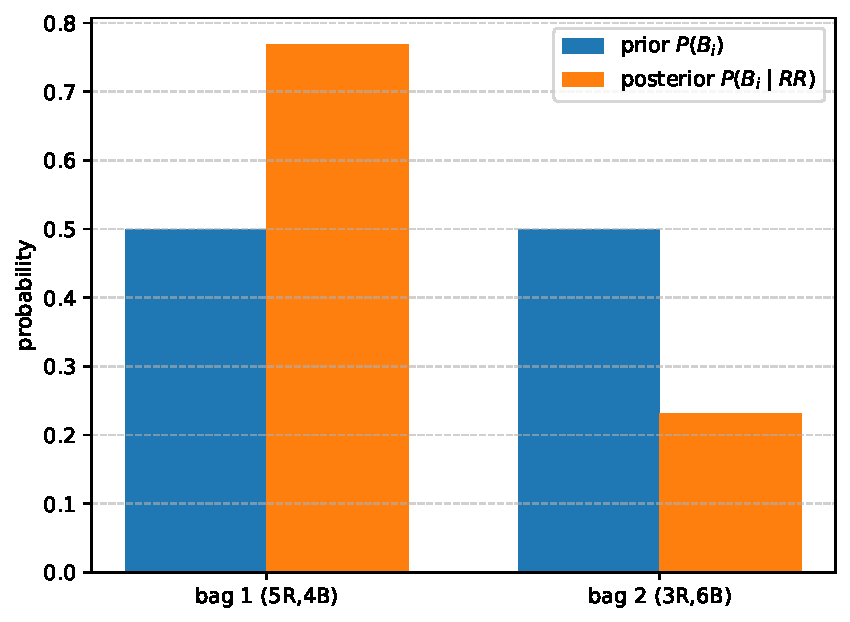
\includegraphics[width=0.70\linewidth]{figs/cbXIIq32.pdf}
    \caption{Prior and posterior probabilities of the two bags}
    \label{fig:EE26BTECH11218-cb12_q32}
\end{figure}
\item If the area between the curves $x=y^2$ and $x=4$ is divided into two equal parts by the line $x=a$, then find the value of $a$ using integration.
\hfill (CBSE~XII~\cbxiiyear)
\\
\solution
From \eqref{eq:EE26BTECH11218-cb12-area}, the total area is $A\brak{4}=\frac{4}{3}\cdot4^{3/2}=\frac{32}{3}$. The line $x=a$ halves it iff
\begin{align}
A\brak{a} = \frac{4}{3}a^{3/2} = \frac{1}{2}\cdot\frac{32}{3} \implies a^{3/2} = 4
\end{align}
\begin{align}
\therefore a = 4^{2/3} = 2^{4/3} \approx 2.52
\end{align}
The following code solves $A\brak{a}=\frac{1}{2}A\brak{4}$ numerically and verifies this in \figref{fig:EE26BTECH11218-cb12_q35a}.
\begin{lstlisting}[frame=single, basicstyle=\rmfamily, escapeinside={(*@}{@*)}]
(*@\makebox[\dimexpr\linewidth-2\fboxsep-2\fboxrule\relax][c]{codes/cbXIIq35a.py}@*)
\end{lstlisting}
\begin{figure}[H]
    \centering
    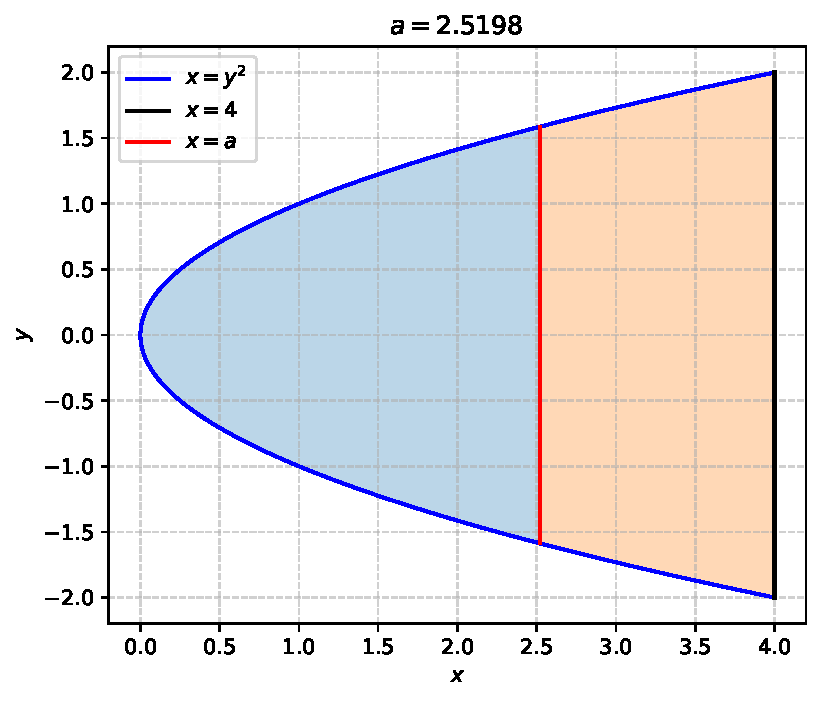
\includegraphics[width=0.70\linewidth]{figs/cbXIIq35a.pdf}
    \caption{Region between $x=y^2$ and $x=4$ divided equally by $x=a$}
    \label{fig:EE26BTECH11218-cb12_q35a}
\end{figure}
\item Find $\displaystyle\int\frac{x}{\brak{x-1}^2\brak{x+2}}dx$.
\hfill (CBSE~XII~\cbxiiyear)
\\
\solution
From \eqref{eq:EE26BTECH11218-cb12-partial}, $x = A\brak{x-1}\brak{x+2}+B\brak{x+2}+C\brak{x-1}^2$. Matching the coefficients of $x^2$, $x$ and $1$,
\begin{align}
\myvec{1 & 0 & 1 \\ 1 & 1 & -2 \\ -2 & 2 & 1}\myvec{A \\ B \\ C} = \myvec{0 \\ 1 \\ 0} \implies \myvec{A \\ B \\ C} = \myvec{\frac{2}{9} \\ \frac{1}{3} \\ -\frac{2}{9}}
\end{align}
Hence
\begin{align}
\int\frac{x\,dx}{\brak{x-1}^2\brak{x+2}} = \frac{2}{9}\ln\abs{x-1}-\frac{1}{3\brak{x-1}}-\frac{2}{9}\ln\abs{x+2}+c
\end{align}
The following code verifies this, including $\int_2^5=0.4337$ against the antiderivative, in \figref{fig:EE26BTECH11218-cb12_q35b}.
\begin{lstlisting}[frame=single, basicstyle=\rmfamily, escapeinside={(*@}{@*)}]
(*@\makebox[\dimexpr\linewidth-2\fboxsep-2\fboxrule\relax][c]{codes/cbXIIq35b.py}@*)
\end{lstlisting}
\begin{figure}[H]
    \centering
    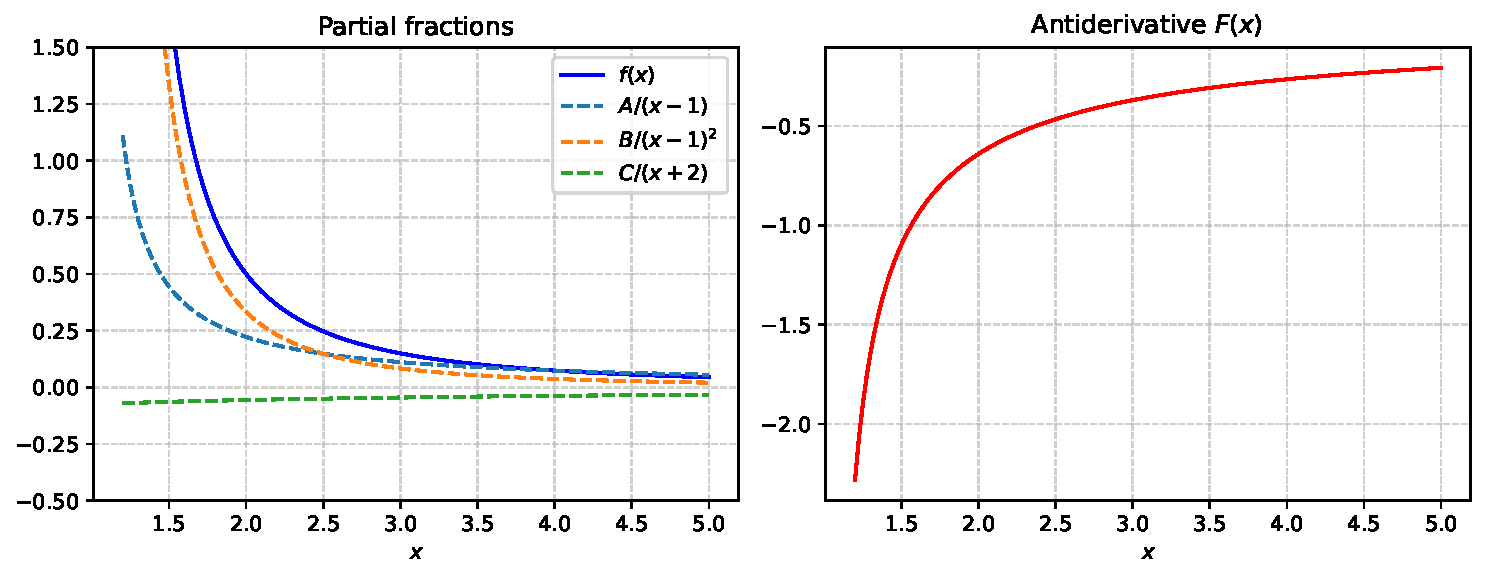
\includegraphics[width=0.95\linewidth]{figs/cbXIIq35b.pdf}
    \caption{Partial fractions of the integrand and its antiderivative}
    \label{fig:EE26BTECH11218-cb12_q35b}
\end{figure}
\end{enumerate}
